\section{Legacy Invoice}\label{sec:legacy-invoice}

This chapter focuses on the existing implementation of the invoice template in GinVoice and the need to upgrade it to a more flexible and automated solution using \pkg{lua-placeholders}.
We will examine the current \LaTeX\ template of the invoice and identify which parts of it can be replaced.
Additionally, we will analyze the structure of the invoice data and discuss why certain parts are split.
Finally, we will discuss the limitations of the current system and emphasize the benefits of transitioning to \pkg{lua-placeholders}.
The use of \pkg{lua-placeholders} will be discussed in more detail in the following chapter.
This change enables us to create a more efficient and flexible invoicing solution that is fully integrated into the \LaTeX\ domain.

\subsection{\LaTeX\ Template}
It is important to note that GinVoice\cite{ginvoice} currently uses a Python script -- \texttt{generator.py} -- to generate additional \TeX\ files.
These \TeX\ files are then included in the template using \cs{include}, so that the necessary macros are available.
However, with the introduction of \pkg{lua-placeholders}, this approach will no longer be necessary.
Below is an example of the code within the \texttt{document} environment:

\lstinputlisting[name=invoice-original,language={[LaTeX]TeX},firstnumber=52,linerange={52-81},numbers=left,xleftmargin=15pt]{ginvoice/invoice-original.tex}

The above code demonstrates various macros that will be replaced by \pkg{lua-placeholders}, including \cs{title}, \cs{subtitle}, \cs{addressee}, \cs{customer\-info}, \cs{supplierinfo}, \cs{tablefooter}, \cs{tablereco\-rds}, \cs{theending}, and \cs{images}.
Additionally, there are variables such as style-related information and \cs{currency} that will also be addressed.

\subsection{Invoice Data}\label{sec:invoice data}
\begin{figure}[!ht]
    \centering
    \begin{tikzpicture}
    \begin{class}[text width=5cm]{Invoice}{1.75,0}
        \attribute{title : String = Invoice}
        \attribute{subtitle : String}
        \attribute{currency : String = \cs{EUR}}
        \attribute{number : Number}
        \attribute{date : String = \cs{today}}
        \attribute{records : Table}
        \attribute{totals : Table/Object}
        \attribute{ending : String}
    \end{class}
    \begin{class}[text width=3cm]{Supplier}{3.5,-4.75}
        \attribute{email : String}
        \attribute{website : String}
        \attribute{accountnr : String}
    \end{class}
    \begin{class}[text width=3cm]{Client}{0,-4.75}
        \attribute{name : String}
        \attribute{street : String}
        \attribute{postal : String}
        \attribute{place : String}
    \end{class}
    \begin{class}[text width=4cm]{Style}{3,-7.5}
        \attribute{images : List}
        \attribute{main font : String}
        \attribute{mono font : String}
        \attribute{foreground color : String}
        \attribute{background color : String}
        \attribute{\sout{colored table} : Boolean}
    \end{class}
    \draw[umlcd style, diamond-angle 45] ($(Invoice.south west) - (-1.25,0)$) -- ($(Client.north) + (.375,0)$);
    \draw[umlcd style, diamond-angle 45] ($(Invoice.south east) + (-1.25,0)$) -- ($(Supplier.north) + (-.375,0)$);
    \draw[umlcd style, diamond-angle 45] ($(Supplier.south) + (-.375,0)$) -- ($(Style.north) + (.125,0)$);
\end{tikzpicture}

    \caption{Class Diagram of the Invoice}\label{fig:invoice-cd}
\end{figure}
\noindent
The invoice is divided into separate parts to specify the necessary information per customer or supplier.
For \LaTeX\ users, there are alternative \LaTeX\ packages available such as \texttt{invoice} and \texttt{invoice2}, which include arithmetic functionalities such as total amounts and grand totals.
Therefore, it is possible to make the interface even simpler, but this is not a goal within this article.
Furthermore, certain parts such as the title, subtitle, and currency symbol may be better handled at the level of the supplier or customer, as they often vary per supplier or customer.

Finally, all styling-related solutions are currently included in the invoice data, but for \LaTeX\ users, this is unnecessary as they can make these adjustments directly in \LaTeX\ itself.

\subsection{Example Output}
\begin{figure}[!ht]
    \centering
    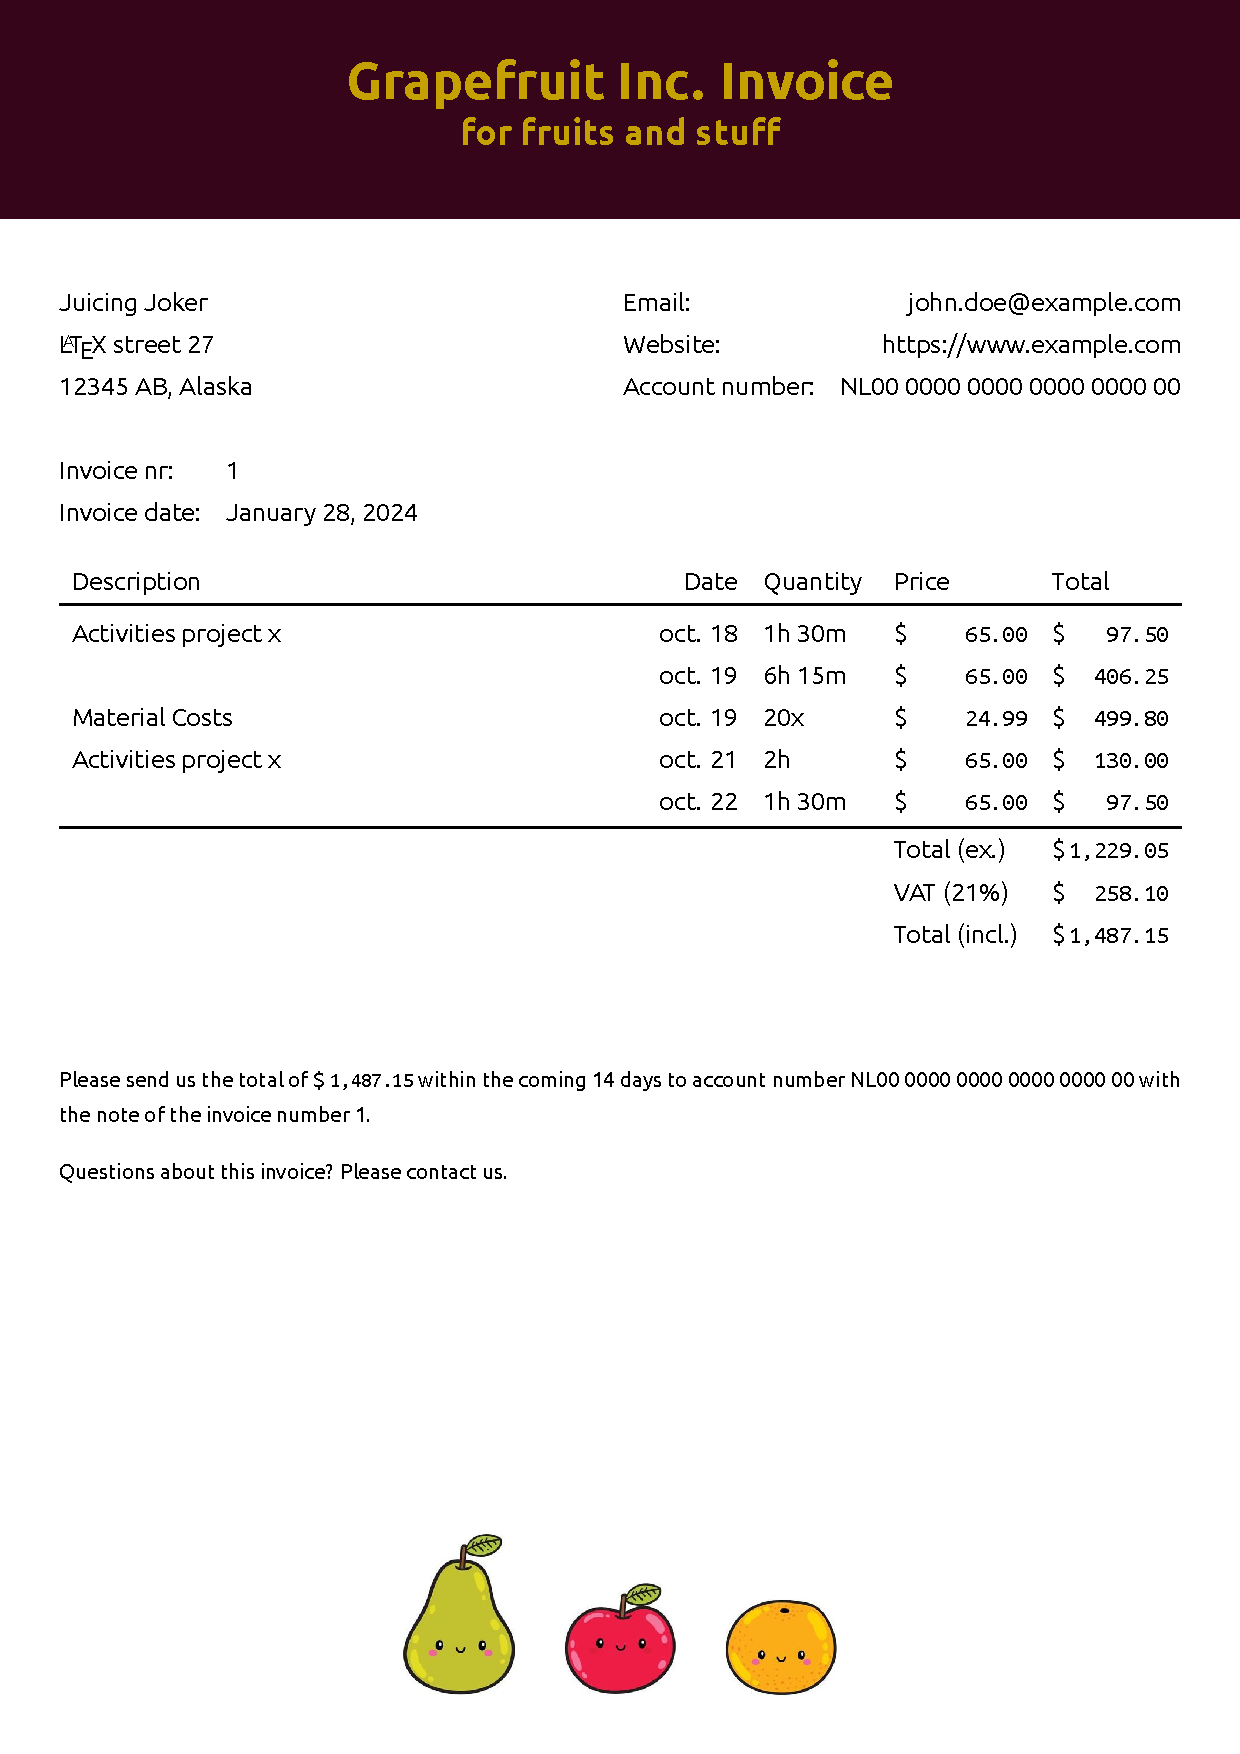
\includegraphics[width=\linewidth]{ginvoice/ginvoice.pdf}
    \caption{Example invoice generated with GinVoice}
    \label{fig:voorbeeldfactuur}
\end{figure}

The example in Figure~\ref{fig:voorbeeldfactuur} shows an invoice generated using the current implementation of GinVoice.
However, currently generating this example requires Python, which is undesirable for template makers who primarily use \LaTeX.
